\documentclass[11pt,aspectratio=169]{beamer}
\usepackage{hp-dfr-slides}
\graphicspath{{../../../assets/}}

\title{The theory}
\subtitle{The error representation and the bound, with proofs}
\author{Carlos Vera-Ciro}
\institute{Goal-Oriented DFR series \textbar\ Part 3}
\date{}

\begin{document}

\begin{frame}[plain,noframenumbering]
  \titlepage
\end{frame}

% =============================================================================
\begin{frame}{What we will establish}
  Everything is elementary: a few lines of functional analysis, no
  regularity assumed beyond well-posedness.
  \medskip
  \begin{enumerate}\itemsep0.5em
    \item The \important{setting}: trial and test spaces, the bilinear form, the
          two hypotheses (Banach--Necas--Babuska).
    \item The \important{DFR error-loss equivalence}, derived.
    \item The \important{exact error representation} for the QoI (a proposition,
          with proof).
    \item The \important{main bound}: the QoI error is controlled by the goal
          loss plus a computable remainder (a theorem, with proof).
    \item Two \important{remarks}: the second-order structure, and how standard
          DFR is recovered.
  \end{enumerate}
\end{frame}

% =============================================================================
\section{The setting}
% =============================================================================

\begin{frame}{Spaces, form, and the primal problem}
  Let $U$ (trial) and $V$ (test) be Hilbert spaces, $a : U \times V \to \R$ a
  bilinear form, and $\ell \in V^*$.
  \medskip
  \begin{block}{Primal problem}
    Find $u^* \in U$ with $\quad a(u^*, v) = \ell(v) \quad \forall v \in V.$
  \end{block}
  \medskip
  For $w \in U$, the \important{residual functional} $\Res(w) \in V^*$ is
  \[
    \Res(w)(v) = \ell(v) - a(w, v).
  \]
  Then $\Res(u^*) = 0$, and subtracting the primal problem,
  \[
    \boxed{\;\Res(w)(v) = a(u^* - w,\, v) \quad \forall v \in V\;}
  \]
  the identity every proof below leans on.
\end{frame}

% -----------------------------------------------------------------------------
\begin{frame}{The two hypotheses}
  \begin{block}{(A1) Boundedness}
    $|a(w,v)| \le M\,\norm{w}_U \norm{v}_V$ for all $w \in U$, $v \in V$.
  \end{block}
  \begin{block}{(A2) Inf-sup stability}
    There is $\gamma > 0$ with
    \[
      \inf_{w \ne 0}\sup_{v \ne 0} \frac{a(w,v)}{\norm{w}_U\norm{v}_V} \ge \gamma
      \quad\text{and}\quad
      \inf_{v \ne 0}\sup_{w \ne 0} \frac{a(w,v)}{\norm{w}_U\norm{v}_V} \ge \gamma .
    \]
  \end{block}
  \medskip
  \begin{itemize}\itemsep0.4em
    \item These are the Banach--Necas--Babuska (BNB) hypotheses; they make the
          primal problem and its adjoint well posed.
    \item For the model problem (Poisson, $U = V = H^1_0$, energy norm) they hold
          with $\gamma = M = 1$.
  \end{itemize}
\end{frame}

% -----------------------------------------------------------------------------
\begin{frame}{The DFR error-loss equivalence}
  \begin{theorem}[Error-loss equivalence]
    Under (A1)--(A2), for every $w \in U$,
    \[
      \frac{1}{M}\,\norm{\Res(w)}_{V^*}
        \;\le\; \norm{u^* - w}_U
        \;\le\; \frac{1}{\gamma}\,\norm{\Res(w)}_{V^*} .
    \]
  \end{theorem}
  \begin{proof}
    From the boxed identity, $\norm{\Res(w)}_{V^*} = \sup_{v \ne 0}
    \frac{a(u^*-w,\,v)}{\norm{v}_V}$. The \important{upper} bound on
    $\norm{\Res(w)}_{V^*}$ is (A1) with $w \mapsto u^*-w$, giving
    $\norm{\Res(w)}_{V^*} \le M\norm{u^*-w}_U$. The \important{lower} bound is the
    first inf-sup of (A2) applied to $u^*-w$:
    $\gamma\norm{u^*-w}_U \le \sup_v a(u^*-w,v)/\norm{v}_V = \norm{\Res(w)}_{V^*}$.
    Rearranging gives both inequalities. \qedhere
  \end{proof}
\end{frame}

% =============================================================================
\section{The quantity of interest and its adjoint}
% =============================================================================

\begin{frame}{The QoI and the adjoint problem}
  Let the quantity of interest be a bounded linear functional $J \in U^*$.
  \medskip
  \begin{block}{Adjoint problem}
    Find $z^* \in V$ with $\quad a(w, z^*) = J(w) \quad \forall w \in U.$
  \end{block}
  \medskip
  Well posed by (A1) and the \emph{second} inf-sup of (A2). For $z \in V$, the
  \important{adjoint residual} $\Resad(z) \in U^*$ is
  \[
    \Resad(z)(w) = J(w) - a(w, z).
  \]
  Then $\Resad(z^*) = 0$, and subtracting the adjoint problem,
  \[
    \boxed{\;\Resad(z)(w) = a(w,\, z^* - z) \quad \forall w \in U.\;}
  \]
  \takeaway{Same structure as the primal, with the roles of the two arguments of
  $a$ swapped.}
\end{frame}

% =============================================================================
\section{The error representation}
% =============================================================================

\begin{frame}{Exact error representation}
  \begin{proposition}
    For $u^*$ solving the primal and $z^*$ the adjoint, and \emph{any}
    $u_h \in U$, $z_h \in V$,
    \[
      J(u^*) - J(u_h)
        \;=\; \Res(u_h)(z^*)
        \;=\; \Res(u_h)(z_h) + \Res(u_h)(z^* - z_h) .
    \]
  \end{proposition}
  \begin{proof}
    Take $w = u^* - u_h$ in the adjoint problem, then use the primal identity:
    \[
      J(u^*) - J(u_h) = J(u^* - u_h)
        = a(u^* - u_h,\, z^*)
        = \Res(u_h)(z^*).
    \]
    The second equality is the split $z^* = z_h + (z^* - z_h)$ and linearity of
    $\Res(u_h)$. \qedhere
  \end{proof}
  \medskip
  The first term is computable: it is the goal loss $\QoI = |\Res(u_h)(z_h)|$. The
  second involves the unknown $z^*$, and we bound it next.
\end{frame}

% =============================================================================
\section{The main bound}
% =============================================================================

\begin{frame}{QoI error control}
  \begin{theorem}
    Under (A1)--(A2), for every $u_h \in U$ and $z_h \in V$,
    \[
      \bigl| J(u^*) - J(u_h) \bigr|
        \;\le\;
        \QoI(u_h, z_h)
        \;+\;
        \frac{1}{\gamma}\,\norm{\Res(u_h)}_{V^*}\,\norm{\Resad(z_h)}_{U^*} .
    \]
  \end{theorem}
  \medskip
  \begin{itemize}\itemsep0.4em
    \item All three terms on the right are exactly what training minimizes.
    \item The remainder is a \important{product} of the two residuals: second
          order when both are small.
    \item \alert{One-sided}: a reliability bound, not an equivalence. We prove it
          on the next two slides.
  \end{itemize}
\end{frame}

% -----------------------------------------------------------------------------
\begin{frame}{Proof, part 1: split and bound by the dual norm}
  By the error representation and the triangle inequality,
  \[
    |J(u^*) - J(u_h)|
      \;\le\; \underbrace{|\Res(u_h)(z_h)|}_{=\ \QoI(u_h,z_h)}
      \;+\; |\Res(u_h)(z^* - z_h)| .
  \]
  \medskip
  For the remainder, the definition of the dual norm gives
  \[
    |\Res(u_h)(z^* - z_h)|
      \;\le\; \norm{\Res(u_h)}_{V^*}\,\norm{z^* - z_h}_V .
  \]
  \medskip
  It remains to control $\norm{z^* - z_h}_V$ by the \emph{adjoint} residual. That
  is where the second inf-sup enters.
\end{frame}

% -----------------------------------------------------------------------------
\begin{frame}{Proof, part 2: inf-sup on the adjoint error}
  Apply the second inf-sup of (A2) to $z^* - z_h \in V$, then the boxed adjoint
  identity:
  \[
    \gamma\,\norm{z^* - z_h}_V
      \;\le\; \sup_{w \ne 0} \frac{a(w,\, z^* - z_h)}{\norm{w}_U}
      \;=\; \sup_{w \ne 0} \frac{\Resad(z_h)(w)}{\norm{w}_U}
      \;=\; \norm{\Resad(z_h)}_{U^*} .
  \]
  \medskip
  Chaining the three displays,
  \[
    |J(u^*) - J(u_h)|
      \;\le\; \QoI(u_h, z_h)
      \;+\; \frac{1}{\gamma}\,\norm{\Res(u_h)}_{V^*}\,\norm{\Resad(z_h)}_{U^*} .
      \qquad\qedsymbol
  \]
  \takeaway{The bound is fully a posteriori: every term is computed from the two
  trained networks.}
\end{frame}

% -----------------------------------------------------------------------------
\begin{frame}{A corollary: adjoint trained to tolerance}
  \begin{corollary}
    If $\norm{\Resad(z_h)}_{U^*} \le \varepsilon$, then
    \[
      |J(u^*) - J(u_h)|
        \;\le\; \QoI(u_h, z_h) + \frac{\varepsilon}{\gamma}\,\norm{\Res(u_h)}_{V^*}
        \;\le\; \QoI(u_h, z_h) + \frac{M\varepsilon}{\gamma}\,\norm{u^* - u_h}_U .
    \]
  \end{corollary}
  \medskip
  \begin{itemize}\itemsep0.4em
    \item The last step uses the \emph{left} inequality of the DFR equivalence,
          $\norm{\Res(u_h)}_{V^*} \le M\,\norm{u^*-u_h}_U$.
    \item Once the adjoint is accurate, the QoI error is the goal loss plus a
          term that scales with the primal energy error.
  \end{itemize}
\end{frame}

% =============================================================================
\section{Two remarks}
% =============================================================================

\begin{frame}{Remark: second-order structure, and what it does not say}
  If both networks reach energy accuracy $O(\delta)$, the remainder is
  $O(\delta^2)$: driving the goal loss to zero leaves a QoI error quadratic in
  $\delta$. But:
  \medskip
  \begin{itemize}\itemsep0.45em
    \item[\alert{1.}] It \important{presupposes $\delta$ small}, i.e. both networks
          well resolved. In a resolution-limited regime, $\delta$ is not small and
          the bound is weak exactly where the method is wanted.
    \item[\alert{2.}] There is \important{no Galerkin orthogonality} here. The goal
          loss enforces one scalar condition, not orthogonality against a whole
          subspace.
    \item[\alert{3.}] So $\QoI$ is \important{not an estimator}: training drives it
          to zero, and the bound is carried by the remainder. Empirically $\QoI
          \approx 10^{-10}$ while the error $\approx 10^{-5}$.
  \end{itemize}
\end{frame}

% -----------------------------------------------------------------------------
\begin{frame}{Remark: standard DFR is the worst case over goals}
  Take the supremum of the error representation over all unit goals. Since
  \[
    \sup_{\norm{J}_{U^*} = 1} J(u^* - u_h) = \norm{u^* - u_h}_U ,
  \]
  the worst case over goals reproduces the DFR equivalence.
  \medskip
  \begin{itemize}\itemsep0.5em
    \item Standard DFR controls \emph{every} quantity of interest at once.
    \item Goal-oriented DFR controls a \emph{single} prescribed goal.
    \item That is why the latter can be cheaper for a fixed target accuracy: it
          does not pay for the goals you do not care about.
  \end{itemize}
\end{frame}

% =============================================================================
\section{The bound, empirically}
% =============================================================================

\begin{frame}{The bound, verified}
  \begin{columns}[T]
    \begin{column}{0.54\textwidth}
      \begin{center}
        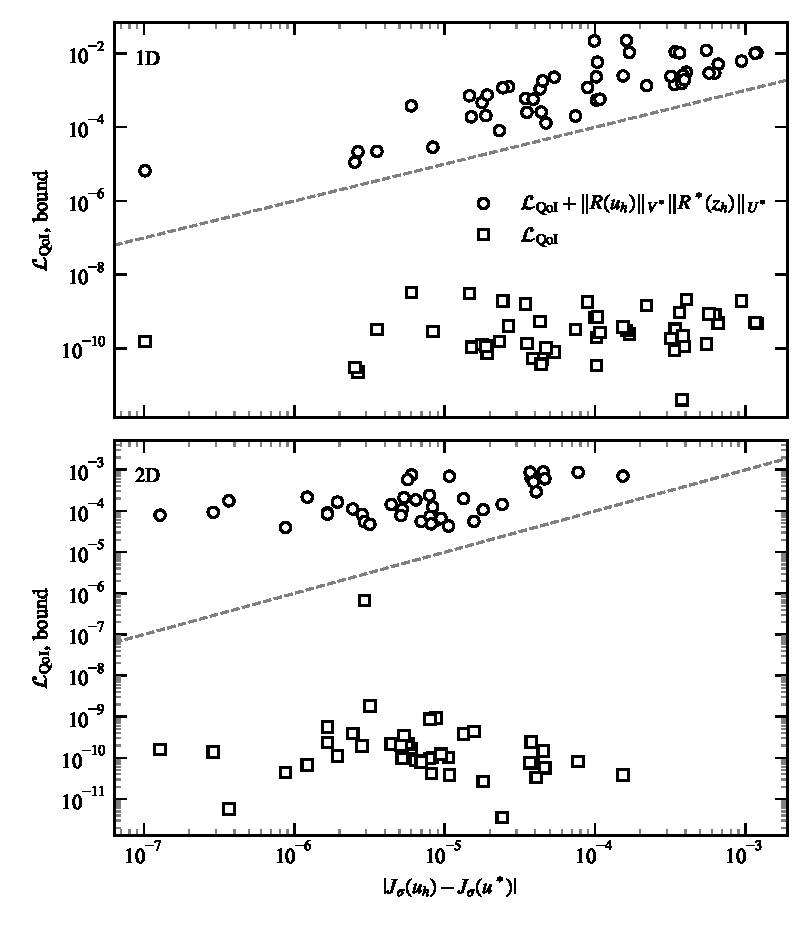
\includegraphics[height=0.72\textheight]{bound-verification}
      \end{center}
    \end{column}
    \begin{column}{0.44\textwidth}
      \vspace{1.2em}
      \begin{itemize}\itemsep0.7em
        \item Circles (the bound) sit \good{above} the diagonal on all 168 runs,
              at about $15\times$ the true error. Never optimistic, despite mode
              truncation and quadrature error.
        \item Squares (the goal loss alone) sit far \alert{below}: it cannot serve
              as an estimator, just as the remark warned.
      \end{itemize}
    \end{column}
  \end{columns}
  \takeaway{The theory is confirmed: a computable, reliable bound, carried by its
  remainder.}
\end{frame}

\end{document}
